\documentclass[a4paper,12pt,twoside,openright]{report}

\usepackage[pdfborder={0 0 0}]{hyperref}    % turns references into hyperlinks
\usepackage[margin=25mm]{geometry}  % adjusts page layout
\usepackage{graphicx}  % allows inclusion of PDF, PNG and JPG images
\usepackage{verbatim}
\usepackage{pdfpages}  % to embed proposal at the end of the dissertation
\usepackage{textcomp}

\renewcommand{\baselinestretch}{1.1}    % adjust line spacing to make
% more readable

\begin{document}
	
	%%%%%%%%%%%%%%%%%%%%%%%%%%%%%%%%%%%%%%%%%%%%%%%%%%%%%%%%%%%%%%%%%%%%%%%%
	% Title
	
	
	\pagestyle{empty}
	
	\rightline{\LARGE \textbf{Peter Lotts}}
	
	\vspace*{60mm}
	\begin{center}
		\Huge
		\textbf{Adding network subsystem provenance collection to CADETS} \\[5mm]
		Computer Science Tripos -- Part II \\[5mm]
		Downing College \\[5mm]
		\today  % today's date
	\end{center}
	
	%%%%%%%%%%%%%%%%%%%%%%%%%%%%%%%%%%%%%%%%%%%%%%%%%%%%%%%%%%%%%%%%%%%%%%%%%%%%%%
	% Proforma, table of contents and list of figures
	
	\pagestyle{plain}
	
	\chapter*{Proforma}
	
	{\large
		\begin{tabular}{ll}
			Name:               & \bf Peter Lotts                       \\
			College:            & \bf Downing College                     \\
			Project Title:      & \bf Adding network subsystem provenance \\
								& \bf collection to CADETS \\
			Examination:        & \bf Computer Science Tripos -- Part II, 2018  \\
			Word Count:         & \bf tbc\footnotemark[1]  \\
			Project Originator: & Dr R.~Sohan                    \\
			Supervisor:         & Dr G.~Jenkinson                    \\ 
		\end{tabular}
	}
	\footnotetext[1]{This word count was computed at [date]	by the provided online tool at \texttt{URL}
	}
	\stepcounter{footnote}
	
	
	\section*{Original Aims of the Project}
	
	To provide additional metadata collection tools for network packets to the Computer Laboratory's existing CADETS project. This will be provided by tracking individual packets as they flow through the network stack of the FreeBSD\footnote{\texttt{http://www.freebsd.org/}} kernel, and making information regarding memory locations used and the time taken by each layer to process a given packet available to DTrace\footnote{\texttt{http://dtrace.org/}}. DTrace is a generic Dynamic Tracing framework which is the primary data collection tool used by the CADETS project to bring kernel data into userspace for analysis. The performance impact of the project on network packet delivery is to be evaluated.
	
	
	\section*{Work Completed}
	
	\textit{What we actually did.}
	
	\section*{Special Difficulties}
	
	None. [We hope!!]
	
	\newpage
	\section*{Declaration Of Originality}
	
	I, Peter Lotts of Downing College, being a candidate for Part II of
	the Computer Science Tripos, hereby declare
	that this dissertation and the work described in it are my own work,
	unaided except as may be specified below, and that the dissertation
	does not contain material that has already been used to any substantial
	extent for a comparable purpose.
	
	\bigskip
	\leftline{Signed [signature]}
	
	\medskip
	\leftline{Date [date]}
	
	\tableofcontents
	
	\listoffigures
	
	%%%%%%%%%%%%%%%%%%%%%%%%%%%%%%%%%%%%%%%%%%%%%%%%%%%%%%%%%%%%%%%%%%%%%%%
	% now for the chapters
	
	\pagestyle{headings}
	
	\chapter{Introduction}
	
	\section{Use Case}
	
	In this project I am evaluating the application of fine-grained tracing within the network stack of the FreeBSD kernel by implementing additional statically defined DTrace probes which are able to provide a platform for both security and performance analysis.
	
	The security aspect of the tool is most useful in combating Advanced Persistent Threats (APTs)\cite{Tankard-APT}, where the attacker slowly infiltrates the target system, hiding out of sight until they can exploit knowledge gained to access the enterprise’s internal network. This may allow the attacker to extract sensitive data from databases in such a way that the access is very hard to distinguish from normal access. Eventually, it is likely that the malware will make a mistake and trigger an indicator of compromise to be observed by administrators, but by then it is difficult to tell what data the malware has seen.
	
	The Computer Laboratory has a project which is trying to combat this by building CADETS\cite{CADETS-main} on top of the FreeBSD operating system, which tracks the provenance of data by collecting metadata from computers all over the network about what processes act on what data and when. This metadata is then collected in a distributed database, where it can be analysed to trace data flows throughout the computer system.
	
	My project adds support for collecting metadata on network packets as they flow through the kernel	network stack. The data collected will allow users of CADETS to seek out suspicious activity which may be being used to attack a system, and will be able to provide a list of locations in kernel memory where packet data were stored. The latter allows a system administrator to infer what data may have been leaked if they are able to determine that some malicious code had access to a particular set of kernel memory addresses.
	
	The performance analysis platform is provided by DTrace's provision of high-accuracy timestamps on probe firing, which when they are collated for a given packet allow the time spent in each section of the network stack to be evaluated. This could be assessed by system administrators, and may allow for better fine-tuning of protocol parameters, some of which are notoriously difficult to set.
	
	\section{The Network Stack}
	
	Almost all modern general purpose computer networks (including, significantly, the Internet) are built upon a layering of several protocols on top of each-other with well-defined interfaces connecting them, defined by the OSI model\cite{ISO-OSI}. These interfaces are often quite general and so this model allows for different protocols to be used for each layer as desired, somewhat interchangeably; this also provides code separation between modules (i.e. layers) with different duties, and so make implementations of these layers - the so-called `Network Stack' - easier to maintain.
	
	\subsection{Layer 1: Physical}
	The bottom-most layer of the network stack, this layer defines the physical communications medium and how to transmit bit streams over it. Properties such as timing, leading to latency and bandwidth, are mostly defined in this layer, although higher layers are likely to decrease bandwidth somewhat by adding mandatory per-packet header data. Generally these days this layer is 802.11 (`Wi-Fi') or Ethernet, although Ethernet networks generally do not need to handle shared medium communications any more.
	
	\subsection{Layer 2: Data Link}
	This layer defines how data frames are transferred between two physically connected nodes, including any shared medium access arbitration and means of addressing such physically connected nodes.
	
	\subsection{Layer 3: Network}
	Typically implemented by the Internet Protocol (IP), addressing and routing between physical networks is defined here, typically including concepts such as broadcast (all nodes receive message) and multicast (a specific group of nodes receive message). This layer often has to handle problems arising from the underlying layers having a different Maximum Transmission Unit (MTU), such that a large packet may not be able to make the next hp connection as a single packet if it is too large for the next physical network. In IPv4 this is handled using fragmentation, where the large packet is split up into several smaller ones which are then sent separately, and the receiver must keep a copy of fragments it receives until it can re-assemble the whole packet and deliver it to the layer above. IPv6 addresses the problem by dropping the packet and sending a notification back to the sender.
	
	\subsection{Layer 4: Transport}
	This layer is responsible for the reliable delivery of data (if required) across a layer 3 link, and creates the notion of a connection which is opened, used to transmit/receive data, and then closed. This is the most common place for application designers to make a choice about layer implementation - TCP or UDP. TCP (the Transmission Control Protocol) provides reliable, in-order delivery of data to higher layers, along with trying to provide fairness between connections through adaptive transmission rate control to avoid congestion. Its main alternative, UDP (the User Datagram Protocol), does not provide reliable delivery but in removing this feature is often able to operate with lower latency than TCP.
	
	\subsection{UNIX Sockets API}
	Under the UNIX `everything is a file' abstraction, layer 4 connections are provided to user applications through sockets, objects which are opened and closed in a similar manner to files and which yield a file descriptor for I/O operations while the connection is open. This abstraction is provided by the kernel (meaning all layers described previously are implemented either in hardware or the kernel) and used by other kernel components as well as all userspace applications which perform network communication.
	
	\section{Tracing as a Security Tool}
	
	Designing systems which are secure in the face of adversaries is hard. One approach to tackling this is to try to minimise the amount of code (either software or a description of hardware) which is required to maintain security - the Trusted Computing Base. If this is small enough, it can then be implemented in verifiable hardware to provide some form of proof of the system's security.
	
	However, this process is difficult and can be very costly, so most systems are unable to make use of such techniques. Instead, they must rely on well-written software (perhaps reviewed by an expert) and on the protections provided by the operating system in conjunction with CPU hardware. This often works reasonably well, however from time to time vulnerabilities are found in even the systems which are believed to be most secure and well-understood - a topical example being in the Spectre CPU vulnerability. In the face of such vulnerabilities in hardware, the software running on top can be exceptionally well engineered and yet can still be exploited since it relies on the provisions made in hardware.
	
	Tracing for security is essentially an extension of audit trails which are formed for example by logging authentication events on a system, in order to provide security analysts with information to aid the reconstruction of events after some sort of attack has occurred. The tracing in this project extends the process to allow analysts to see which memory locations were used by the network stack in processing a particular data packet, in the hopes of being able to inform an impact assessment of what data may have been leaked in an attack.
	
	\section{Similar Work}
	
	Just need to mention Resourceful? - I haven't used it so far, is it even relevant?
	
	\section{Overall design}
	
	The project is to assign uniquely identifying tags to each packet as it flows through the network stack, noting that packet fragmentation/reassembly will make this more difficult. This will then allow DTrace tracepoints to read the tag on each packet when an interesting operation (broadly speaking, a memory allocation) is performed on it. From here, scripts written in DTrace's D language will be able to forward information to a DTrace consumer to display results and answer user queries.

	
	
	\chapter{Preparation}
	
	\section{Starting Point}
	
	The CADETS project currently has a user-space application which collects metadata on kernel-level	datastructures via libdtrace, translates the metadata to a JSON format for easy interpretation, and	then sends this away for processing (often over the network). It also has an application with a user interface to display the data it has collected.
	
	The FreeBSD kernel provides a means of tagging its main internal structure of interest, namely \verb|struct mbuf| using \verb|struct mbuf_tags|. It is thought that this will be sufficient to tag a packet’s data with an unique identifier in order to track its progress through the kernel’s network stack.
	
	Under Linux, the Resourceful framework is able to collect data from auto-generated tracepoints	within the Linux kernel with relatively low overhead, but it does not currently inspect the network subsystem.
	
	\section{Installing the Development System}
	
	I had no prior experience with FreeBSD usage or development, so the first challenge was to get a system up and running to be used for both development and testing. I decided to host FreeBSD as a virtual machine on my Windows 10 laptop, as it has reasonable performance for compiling code, whilst being portable and allowing me to work on the project wherever I am. The virtual machine was set up using Oracle\texttrademark\ VM VirtualBox\footnote{\texttt{http://www.virtualbox.org/}}, as I have most experience using this virtualisation application.
	
	The FreeBSD website provides preinstalled images\footnote{\texttt{http://www.freebsd.org/where.html\#download}} for various virtual machine types, and I decided to use one of these as a basis due to my inexperience with the operating system. Only slow progress was made during the first few days of using this new operating system, as the preinstalled images have a rather basic toolset available and I had to learn how to use a new package manager, and the FreeBSD `ports' system. Having acclimatised to these, I was able to fork the CADETS custom kernel, build and install it onto the running machine.
	
	\section{FreeBSD kernel study}
	
	The first significant piece of planned project work was to inspect the FreeBSD kernel source code for the network stack, gain some familiarity with it, and note the locations of operations which are of particular interest to the project, either from a packet tagging perspective or from the perspective of packet data being copied to a new memory location.
	
	The study commenced at the point where outgoing packets enter the IP layer of the network stack, namely the top of the \verb|ip_output| function. From here, the packet was followed down through the IP layer, exploring all possible control paths
	\footnote{
		With one or two notable exceptions, namely that
		\begin{itemize}
			\item Berkley Packet Filter (BPF) was considered to be out of scope for the project
			\item IPSec allows arbitrary code to be executed via its `hooks' system, and so this cannot be inspected
		\end{itemize}
	}
	and possible exit routes into lower layers. Once the packets had left to go to device drivers, the study then turned to the \texttt{netisr} system, which is responsible for receiving packets from device drivers in the FreeBSD kernel and handing them on to the appropriate next layer (usually the IP layer) to be processed. From here, packets were followed back up the network stack in a similar manner, up to the end of \verb|ip_input|, where packets leave the IP layer to go to the next layer up.
	
	At this point, it was noticed that the project was getting a little behind schedule and, in a meeting with my supervisor, it was decided that for the moment the project would not look any higher than the IP layer, as there was no significant academic benefit to be gained from continuing up to look at the TCP layer. This could be completed at a later stage in the project if time became available.
	
	DID WE GET TIME FOR THIS?
	
	
	\chapter{Implementation}
	
	
	\chapter{Evaluation}
	
	
	\chapter{Conclusion}
	
	
	
	%%%%%%%%%%%%%%%%%%%%%%%%%%%%%%%%%%%%%%%%%%%%%%%%%%%%%%%%%%%%%%%%%%%%%
	% the bibliography
	\addcontentsline{toc}{chapter}{Bibliography}
	\bibliographystyle{plain}
	\bibliography{refs}
	
	%%%%%%%%%%%%%%%%%%%%%%%%%%%%%%%%%%%%%%%%%%%%%%%%%%%%%%%%%%%%%%%%%%%%%
	% the appendices
	\appendix
	
	
	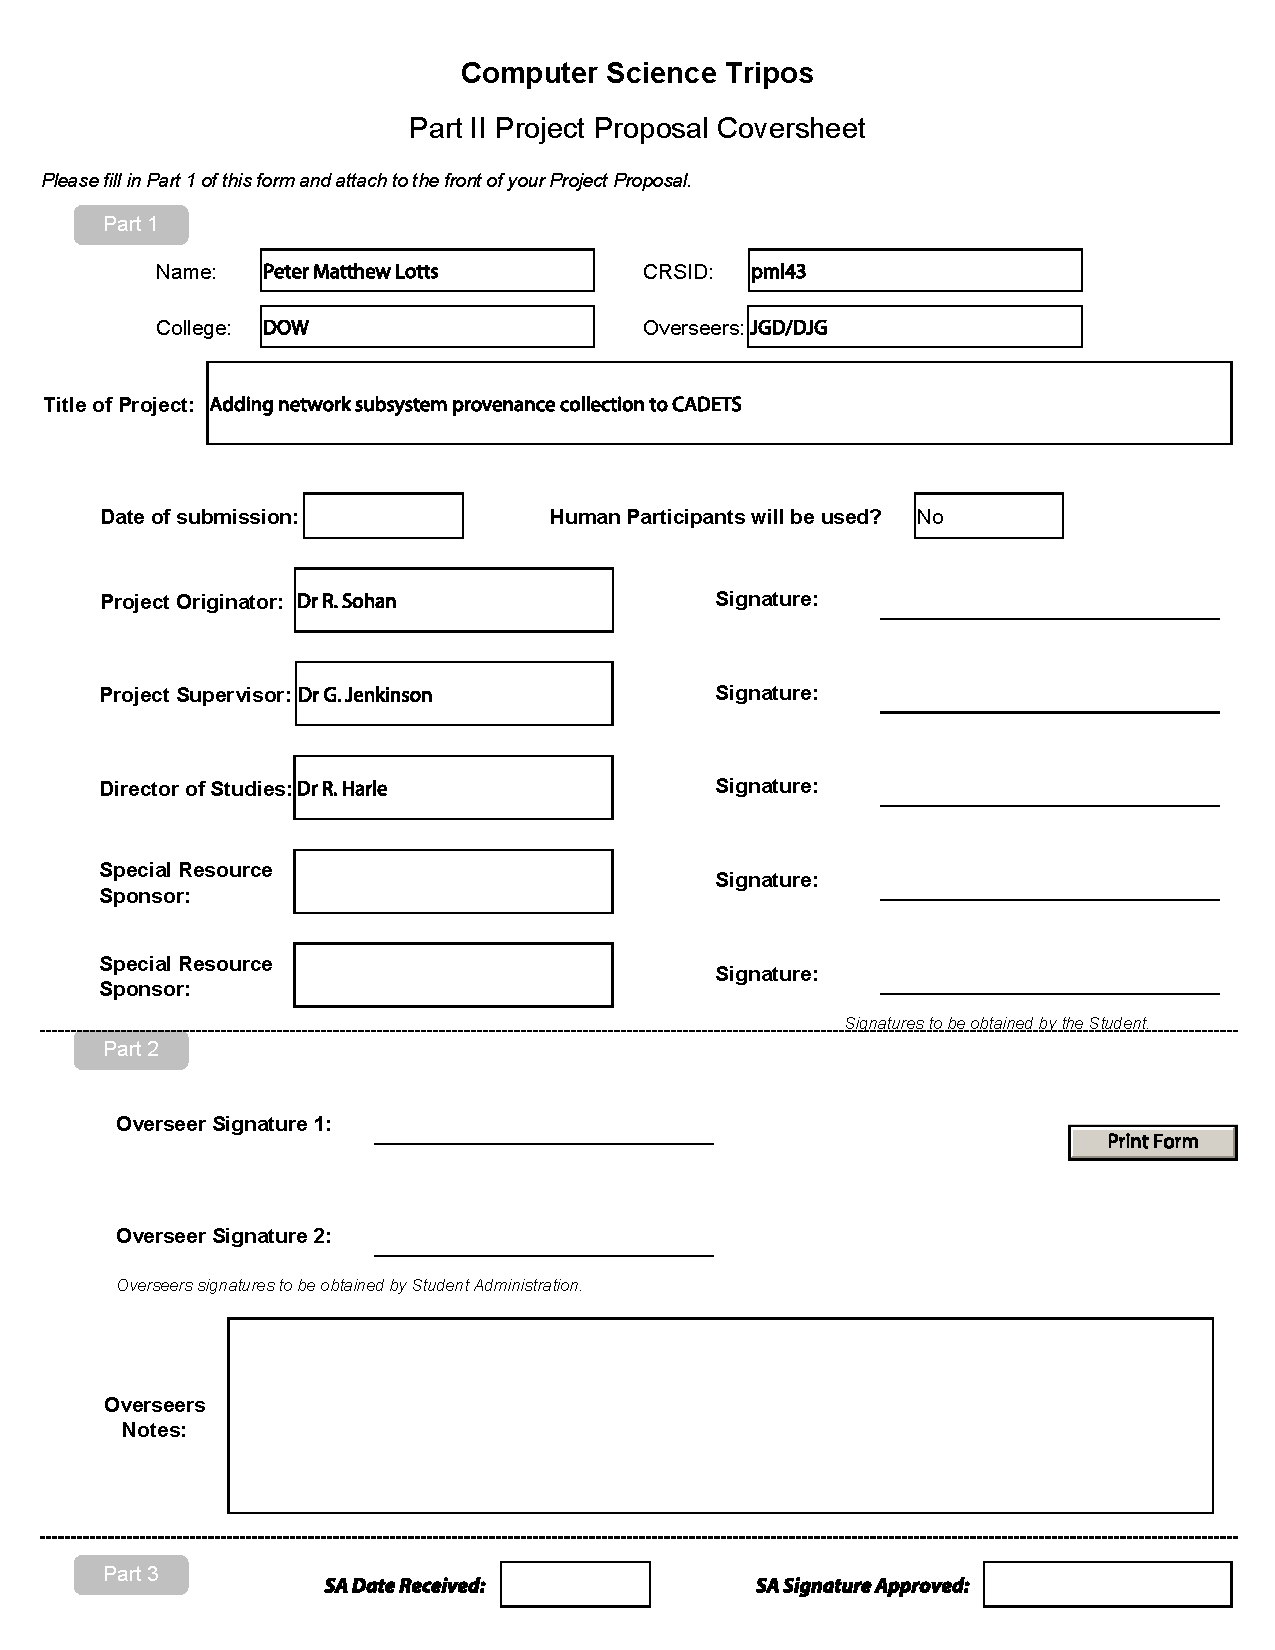
\includepdf{include/Project-Proposal-Cover-Sheet.pdf}
	\includepdf[pages={2-}]{include/Project-Proposal.pdf}
	
	
\end{document}
